\documentclass[A4,12pt, utf8]{article}
\usepackage{tikz}
\usepackage[
    backend=biber,
    style=authoryear-icomp,
    sortlocale=de_DE,
    natbib=true,
    url=false, 
    doi=true,
    eprint=false
]{biblatex}
\usepackage{listings}
\usepackage{xcolor}
\usepackage{hyperref}
\usepackage{tikz}
\usepackage{todonotes}
\usepackage{dirtree}



\newcommand{\tinytodo}[2][]
   {\todo[caption={#2}, size=\small, #1]{\renewcommand{\baselinestretch}{0.5}\selectfont#2\par}}

\colorlet{punct}{red!60!black}
\definecolor{background}{HTML}{EEEEEE}
\definecolor{delim}{RGB}{20,105,176}
\colorlet{numb}{magenta!60!black}

\lstdefinelanguage{json}{
    basicstyle=\normalfont\ttfamily,
    % numbers=left,
    % numberstyle=\scriptsize,
    % stepnumber=1,
    % numbersep=8pt,
    showstringspaces=false,
    breaklines=true,
    frame=lines,
    backgroundcolor=\color{background},
    literate=
     *{0}{{{\color{numb}0}}}{1}
      {1}{{{\color{numb}1}}}{1}
      {2}{{{\color{numb}2}}}{1}
      {3}{{{\color{numb}3}}}{1}
      {4}{{{\color{numb}4}}}{1}
      {5}{{{\color{numb}5}}}{1}
      {6}{{{\color{numb}6}}}{1}
      {7}{{{\color{numb}7}}}{1}
      {8}{{{\color{numb}8}}}{1}
      {9}{{{\color{numb}9}}}{1}
      {:}{{{\color{punct}{:}}}}{1}
      {,}{{{\color{punct}{,}}}}{1}
      {\{}{{{\color{delim}{\{}}}}{1}
      {\}}{{{\color{delim}{\}}}}}{1}
      {[}{{{\color{delim}{[}}}}{1}
      {]}{{{\color{delim}{]}}}}{1},
}
% \addbibresource{linked.bib}

\newcounter{treeline}

\newcommand{\treeroot}[1]{% Title
\node[above] at (0,0) {#1};%
\setcounter{treeline}{0}
}

\newcommand{\treeentry}[2]{% Title, Level
\draw[->] (#2-1,-\value{treeline}/2) -- (#2-1,-\value{treeline}/2-0.5) -- (#2+0.5,-\value{treeline}/2-0.5) node[right] {#1};
\stepcounter{treeline}
}

\newcommand{\altentry}[2]{% Title, Level
\draw[->] (#2-1,-\value{treeline}/2) -- (#2-1,-\value{treeline}/2-0.5) -- (#2+0.5,-\value{treeline}/2-0.5) node[right] {#1};
\foreach \x in {1,...,#2}
{   \draw (\x-1,-\value{treeline}/2) -- (\x-1,-\value{treeline}/2-0.5);
}
\stepcounter{treeline}
}


\title{emuLVC - Stucture of the angularjs app}
\author{Raphael Winkelmann}
\date{\today}
\begin{document}
  % \maketitle

\section{Schematic DB file structure on disc}

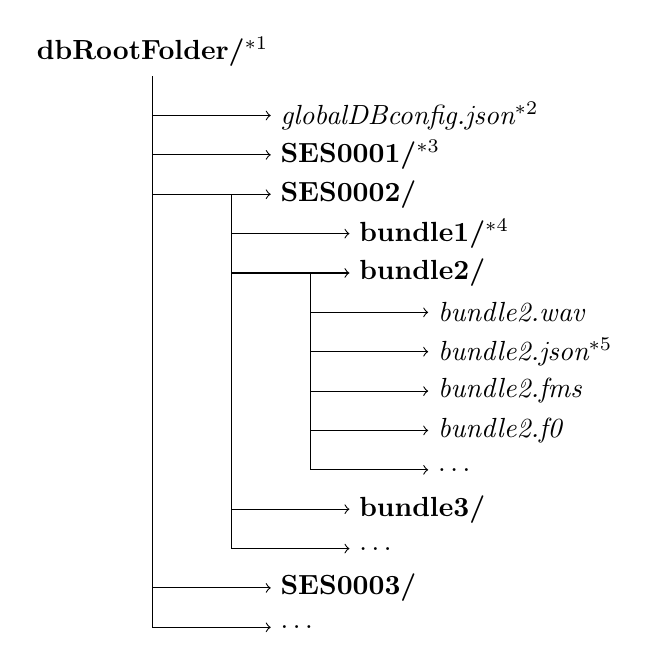
\begin{tikzpicture}
\treeroot{\textbf{dbRootFolder/$^{*1}$}}
\altentry{\textit{globalDBconfig.json$^{*2}$}}{1}
\altentry{\textbf{SES0001/$^{*3}$}}{1}
\altentry{\textbf{SES0002/}}{1}
\altentry{\textbf{bundle1/$^{*4}$}}{2}
\altentry{\textbf{bundle2/}}{2}
\altentry{\textit{bundle2.wav}}{3}
\altentry{\textit{bundle2.json$^{*5}$}}{3}
\altentry{\textit{bundle2.fms}}{3}
\altentry{\textit{bundle2.f0}}{3}
\altentry{\dots}{3}
\altentry{\textbf{bundle3/}}{2}
\altentry{\dots}{2}
\altentry{\textbf{SES0003/}}{1}
\altentry{\dots}{1}
\end{tikzpicture}


\begin{itemize}
  \item $^{*1}$: the name of this folder specifies the name of the database. Is this a good idea? Or should this be defined by the name of $^{*2}$??? Or in a field in $^{*2}$???
  \item $^{*2}$: global config information file (similar to \textit{.tpl} file of old emu). Specifies things like structure of hierarchy and possible views for the DB.
  \item $^{*3}$: Prefix of session folders must be \textbf{SES}. Following this prefix can be anything as long it is unique on a session level (OS won't let you name two folders the same anyway...). If no session is required a dummy session is used called SES0000.
  \item $^{*4}$: a bundle encapsulates what was used to be known as an utterance in a folder. This includes signal files (\textit{wav,SSFF}) and the new annotation file (see $^{*5}$)
  \item $^{*5}$: annotation file containing label information as well as hierarchical information
\end{itemize}




\section{File structure of json files (label+signal)}




\begin{lstlisting}[caption=internal label representation, label=ilr, language=json,firstnumber=1]
{
  "fileURL": "file:/path/to/msajc003.TextGrid",
  "tiers": [
  {"tierName": "Phonetic",
    "type": "seg",
    "events": [
      {"label": "", "startSample": 0, "sampleDur": 8267}, 
      {"label": "V", "startSample": 8268, "sampleDur": 3064}, 
      {"label": "m", "startSample": 11333, "sampleDur": 3670}, 
      ...
    ]
  }
}
\end{lstlisting}

\begin{lstlisting}[caption=internal derived signal representation,label=idsr, language=json,firstnumber=1]
{
  "fileURL": "file:/path/to/msajc003.fms",
  "sampleRate" = 200,
  "origFreq" = 20000,
  "startTime" = 0.0025,
  "columns" = [
  {"name": "fm",
    "length": 4,
    "ssffDataType": "SHORT"
    "values" : [[0, 1042, 2072, 3170],
                [0, 1260, 2122, 3118],
                [0, 1339, 2293, 3258],
                ...]},
  {"name": "bw",
    "length": 4,
    "ssffDataType": "SHORT"
    "values" : [[0, 886, 371, 890],
                [0, 724, 567, 826],
                [0, 410, 664, 740],
                ...]}
  ]
}
\end{lstlisting}

% \printbibliography

% \begin{figure}[h]
%   \tikzstyle{rootscope}=[rectangle, fill=black!50, thick,
%                  inner sep=0.1cm, rounded corners]
%   \tikzstyle{ctrl}=[rectangle, fill=red!50, thick,
%                  inner sep=0.1cm, rounded corners]
%   \tikzstyle{service}=[rectangle, fill=green!50, thick,
%                  inner sep=0.1cm]
%   \tikzstyle{directive}=[rectangle, fill=blue!50, thick,
%                  inner sep=0.1cm, rounded corners]

%   \tikzstyle{jso}=[rectangle, fill=yellow, thick,
%                  inner sep=0.1cm]


%   \begin{tikzpicture}
%   \node (rootscope) at ( 0, 7) [rootscope] {\small{rootscope}};

%     \node (configServ) at ( -6, 2) [service] {\small{ConfigProviderService}};

%     \node (mainCtrl) at ( 0, 5) [ctrl] {\small{mainCtl}};
%     \node (viewState) at ( -4, 5) [service] {\small{viewState}};
%     \node (ioHandler) at ( 4, 6) [service] {\small{Iohandlerservice}};
%     \node (soundHandler) at ( 4, 5) [service] {\small{Soundhandlerservice}};
%       \node (SSFFparser) at ( 7, 7.5) [service] {\small{ssffparserservice}};
%       \node (TextGridParser) at ( 7, 7) [service] {\small{TGParser}};
%       \node (labFileParser) at ( 7, 6.5) [service] {\small{labParser}};
%       \node (Dropbox) at ( 7, 6) [service] {\small{DBHandler}};
%       \node (Socket) at ( 7, 5.5) [service] {\small{Sockethandler}};


%     \node (keys) at ( 0, 4) [ctrl] {\small{handleglobalkeystrokes}};

%     % oscispec ctrl
%     \draw (-1, 3) rectangle (7, -1.5);

%     \node (osciSpecCtrl) at ( 0, 3) [ctrl] {\small{timelineCtrl}};

%     \node (spect) at ( 1, 2) [directive] {\small{$<$spectrogram$>$}};

%           \node (canspect) at (4 , 1) [directive] {\small{$<$canvas handlemouseinspect$>$}};
    
%     \node (osci) at ( 1, 0) [directive] {\small{$<$oscii$>$}};

%           \node (canosci) at (4 , -1) [directive] {\small{$<$canvas handlemouseinosci$>$}};


%     \node (Drawhelperservice) at (8 , 4) [service] {Drawhelperservice};

%     % tiers
%     \draw (-1, -2) rectangle (7, -4.5);
%     \node (ssffData) at ( -4, 3) [jso] {\small{ssffData(model)}};
%     \node (model) at ( -4, -2) [jso] {\small{tierInfos(model)}};
%     \node (tierCtrl) at ( 0, -2) [ctrl] {\small{handletiersCtl}};

%     \node (tier) at ( 1, -3) [directive] {\small{$<$tier$>$}};

%           \node (cantier) at (4 , -4) [directive] {\small{$<$canvas handlemouseintier$>$}};

%     %%%%%%%%%%%%%%%%%%%%%%%%%%%%%%%%%%%%%%%%%%%%
%     %connections
%     \draw [-] (mainCtrl) -- (keys);
%     \draw [-] (keys) -- (osciSpecCtrl);
%     \draw [-] (osciSpecCtrl.west) -- (tierCtrl.west);
%     \draw [<->] (osciSpecCtrl.west) -- (ssffData);
%     \draw [<->] (tierCtrl.west) -- (model);

%     \draw [->, dotted] (ioHandler) -- (mainCtrl);
%     \draw [->, dotted] (soundHandler) -- (mainCtrl);

%     \draw [<-, dotted] (ioHandler) -- (SSFFparser);
%     \draw [<-, dotted] (ioHandler) -- (TextGridParser);
%     \draw [<-, dotted] (ioHandler) -- (labFileParser);
%     \draw [<-, dotted] (ioHandler) -- (Dropbox);
%     \draw [<-, dotted] (ioHandler) -- (Socket);

%     %viewstate
%     \draw [->, dotted] (viewState) -- (mainCtrl);
%     \draw [->, dotted] (viewState) -- (osciSpecCtrl);
%     \draw [->, dotted] (viewState) -- (tierCtrl.west);

%     %configproviderservice
%     \draw [->, dotted] (configServ) -- (osciSpecCtrl.west);
%     \draw [->, dotted] (configServ) -- (tierCtrl.west);
%     \draw [->, dotted] (configServ) -- (keys.west);
%     \draw [->, dotted] (configServ) -- (mainCtrl.west);

%     %Drawhelperservice

%     \draw [->, dotted] (Drawhelperservice) -- (osciSpecCtrl.east);
%     \draw [->, dotted] (Drawhelperservice) -- (tierCtrl.east);

%   \end{tikzpicture}
% \end{figure}
\end{document}